\section{Testy a continuous integration}
W celu lepszego zrozumienia istoty automatyzacji testów konieczne jest najpierw zrozumienie testów samych w sobie. Jak zostało to opisane w rozdziale 1.4 - pisanie testów jest integralną częścią pracy każdego programisty. Wiele osób uważało to dawniej za żmudne zadanie, nieprzynoszące wymiernych korzyści, jednakże z biegiem czasu stało się jasne, że w dużych projektach informatycznych są one konieczne, co widać w dzisiejszych czasach w wypowiedziach wielu osób. \cite{UnitOpinions} \cite{UnitResults}

\subsection{Testy jednostkowe}
Testem jednostkowym nazywa się kod, który jest w stanie wywołać inny fragment kodu programu, a następnie sprawdzić czy działanie tamtego kodu jest zgodne z zakładanym przez programistę działaniem. \cite{UnitDefinition}
\par Autor tej definicji zdefiniował też kilka warunków, które powinien spełniać każdy test jednostkowy dobrej jakości: 
\begin{itemize}
    \item jest w pełni zautomatyzowany - nie wymaga żadnej interakcji od użytkownika
    \item odizolowany od reszty kodu, którego nie sprawdza oraz od innych testów - w celu spełnienia tego warunku często będą wykorzystywane tak zwane "mocki" oraz "stuby" 
    \item nie ma dostępu do baz danych lub plików na dysku
    \item jest deterministyczny, nie zawiera losowych danych, przy każdym uruchomieniu kodu zwraca taki sam rezultat
    \item jest szybki - należy pamiętać, że testów będzie w kodzie dużo, a także będą one często uruchamiane
    \item skupia się na pojedynczym logicznym elemencie programu
    \item czytelny
    \item łatwy w zrozumieniu
    \item wiarygodny - wynika to z dwóch powyższych warunków. Po otrzymaniu wyniku testów nie powinniśmy mieć wątpliwości czy jest on poprawny
\end{itemize}
Fragmentem kodu, który podlega testom jest zwykle najmniejsza jego część, która odpowiada za jedno logiczne działanie. Najczęściej będzie to więc pojedyncza metoda klasy lub cała klasa. 

Odpowiednie przygotowanie testów jest kluczowe jeśli chcemy uniknąć w naszym projekcie regresji - pojawienia się błędów w kodzie, który wcześniej działał poprawnie ( wiąże się to także z innym rodzajem testów - testami regresyjnymi, których zadaniem jest sprawdzanie, czy wprowadzona zmiana w danym miejscu programu nie spowoduje powstania błędów w innych jego miejscach \cite{RegressionTesting}). 

Warto wspomnieć także o testowaniu tak zwanych przypadków brzegowych (Edge cases). W przypadku gdy w kodzie występuje przykładowo porównanie x$>$5, warto sprawdzić jak dana metoda zachowa się z wartościami 4, 5 oraz 6. Innymi warunkami brzegowymi mogą często być (w przypadku gdy typ danych to integer): 
\begin{itemize}
    \item wartość 0
    \item wartość ujemna, często -1
    \item minimalna wartość przewidziana dla funkcji
    \item maksymalna wartość przewidziana dla funkcji
    \item wartość odpowiednio mniejsza i większa od wartości minimalnej i maksymalnej, która powinna spowodować błąd 
\end{itemize}

\subsubsection{Wykorzystanie atrap}
Jak zostało to opisane wcześniej - każdy test jednostkowy powinien być odizolowany od reszty kodu i innych zależności zewnętrznych. Należy to rozumieć poprzez bycie odizolowanym od plików na dysku, danych z internetu, dostępu do baz danych wykorzystywanych w projekcie oraz do klas i interfejsów niebędących przedmiotem testów. Konieczność taka zachodzi z kilku powodów, między innymi: 
\begin{itemize}
    \item test może dać nam zły rezultat, nawet gdy sam fragment, który ma on testować nie zawiera żadnych błędów. Błędy wynikają wtedy z innych zależności, które powinny zostać wykryte przez testy przygotowane specjalnie dla nich
    \item mogą one zajmować zbyt dużo czasu. Szczególnie chodzi tutaj o dostęp do plików na dysku oraz zapytania do bazy danych, które zwykle same w sobie zajmują wielokrotnie więcej czasu niż sam testowany przez nas kod
\end{itemize}

Oczywistym jest, że nawet gdy sam test nie ma mieć dostępu do zależności zewnętrznych, to sam kod musi ten dostęp posiadać w celu prawidłowego działania. Aby móc poprawnie przetestować taki kod, który wymaga różnych zależności zewnętrznych wykorzystujemy atrapy. Wykorzystywane są one wyłącznie przez testy, nie mają żadnego wpływu na działanie programu. Ich zadaniem jest symulowanie działania prawdziwego kodu, który nie podlega naszym testom. W praktyce najczęściej wykorzystywany będzie do tego specjalny framework, np. Moq dla C\#, Mockito dla Java lub unittest.mock dla pythona. 

W literaturze wyznaczonych zostało wiele rodzajów atrap. Znaczna część dostępnych frameworków nie rozdziela ich jednak, a duża część społeczności różnie definiuje poszczególne rodzaje. Warto wymienić kilka najpopularniejszych używanych określeń: 
\begin{itemize}
    \item Stub - najprostszy rodzaj atrapy. Potrafi ona przechowywać dane predefiniowane jej w trakcie pisania testu oraz odpowiedzieć tymi danymi podczas wywołania go. Nadaje się idealnie do symulowania działania bazy danych, która ma zwrócić wartość na podstawie zapytania
    \item Mock - są to obiekty, które mają możliwość otrzymywania danych oraz weryfikowania, czy są one zgodne z oczekiwaniami w danym teście 
    \item Fake - bardziej zaawansowane rodzaje atrap. Posiadają one faktyczne implementacje kodu, zwykle pisane jednak specjalnie pod dany przypadek testowy. Kod ten jest znacznie mniej rozbudowany od produkcyjnego, pozwala jedynie na przetestowanie wymaganej funkcjonalności. 
\end{itemize}

\subsubsection{Przykładowy test jednostkowy}
Do napisania najprostszego testu jednostkowego w języku python nie jest konieczne nawet wykorzystanie żadnego zewnętrznego frameworka. 

\begin{lstlisting}[caption={Test jednostkowy w języku Python}]
string = "asda"

assert isinstance(string, str), "Not string"
assert len(string) > 0, "No text to capitalize"

x = string.upper()
\end{lstlisting}

Wykorzystana została tutaj asercja, która jest podstawą każdego testu jednostkowego. Jej zadaniem jest sprawdzenie czy dana zależność określona w kodzie przez programistę jest spełniona. W tym przypadku wykorzystane zostały dwie asercje. Możliwe jest zrezygnowanie z pierwszej, ponieważ sprawdza ona czy obiekt jest typu string, co zostałoby wykryte później przez funkcję upper(). Istotniejsza jest druga z nich, która sprawdza czy dany string nie jest pusty. Jest to o tyle istotne, że funkcja upper() przyjmuje puste stringi i nie zwróci nam dla nich żadnego błędu. Wykorzystanie takiej asercji powoduje, że programista może w dalszej części kodu zakładać, że wartość, którą otrzyma z funkcji upper() nie będzie pusta. W przypadku użycia pustego łańcucha znaków otrzymamy następujący komunikat: 

\begin{lstlisting}[caption={Błąd asercji podczas testu}]
AssertionError                            Traceback (most recent call last)
<ipython-input-40-7526aaf9a6e8> in <module>
      2 
      3 assert isinstance(string, str), "Not string"
----> 4 assert len(string) > 0, "No text to capitalize"
      5 
      6 x = string.upper()

AssertionError: No text to capitalize
\end{lstlisting}

Użycie dowolnego niepustego łańcucha znaków spowoduje, że test jednostkowy zostanie pomyślnie wykonany i nie zostanie zwrócony żaden błąd. 

\begin{figure}[htbp]
    \centering
    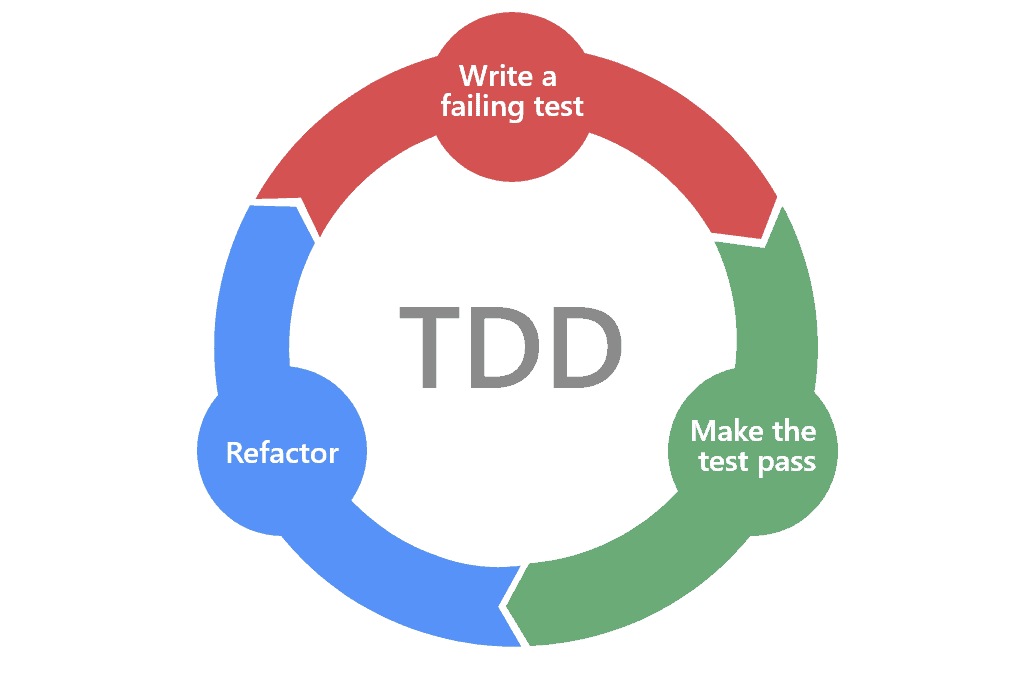
\includegraphics[width=10cm]{images/tdd.png}
    \caption{Zasada Red-Green-Refactor}
    \label{fig:redgreen}
\end{figure}

\subsubsection{Metodyki pisania testów}
\par Najpopularniejsze obecnie są dwie metody pisania testów: 
\begin{itemize}
    \item TDD - Test Driven Development - zaproponowana została przez Kenta Becka w 2002 roku. \cite{TestDrivenDevelopment} Zakłada, że testy będą napędzały tworzenie projektu i stały u jego podstawy. 
    \par Pierwszym krokiem przy implementacji nowej funkcji w naszym projekcie powinno być napisanie samego testu, który oczywiście na początku nie powiedzie się, ponieważ kod, który ma on testować nie został jeszcze napisany. Po napisaniu testu przechodzi się do pisania kodu, który w jak najłatwiejszy sposób będzie w stanie zaliczyć napisany przez nas test. Ostatnim krokiem tego cyklu jest refactoring kodu, polepszający jego jakość samą w sobie, ale bez zmieniania jego funkcjonalności, tak aby spełniał on oczekiwane standardy.
    Takie podejście pozwala na tworzenie dobrze zaprojektowanego kodu, który jest w całości pokryty testami, co owocuje w przyszłości, kiedy konieczne jest wprowadzanie zmian w bazie kodu.
    
    Pozwala to również na wymuszenie na osobach piszących kod, aby był on dobrze przemyślany. Konieczność napisania testu przed implementacją funkcjonalności wymusza na programiście, aby zastanowił się dogłębniej jak ma wyglądać struktura jego kodu oraz co chce on osiągnąć implementując daną klasę. 
    
    Podejście TDD zapewnia więc wiele zalet, ale nie jest ono oczywiście całkowicie pozbawione wad. Jedną z nich jest konieczność nauczenia programistów tej metodologii w przypadku jeśli wcześniej nie mieli z nią do czynienia. Główną wadą jest jednak znacznie zwiększony narzut czasowy na pisanie testów wynikający z wykorzystania TDD. Duże pokrycie kodu testami zajmuje programistom zwykle znacznie więcej czasu niż podczas standardowego implementowania funkcjonalności, a następnie napisania testów dla wybranych wedle uznania fragmentów kodu. Zainwestowany jednak w ten sposób czas zwraca się w późniejszych fazach projektu, jeśli okazuje się, że konieczna jest jakaś zmiana w strukturze kodu. Najwięcej czasu oszczędza się w porównaniu do standardowych metod pisania kodu na poprawianiu błędów działania programu. Wszystkie błędy poprawiane są na bieżąco, nie ma możliwości implementacji funkcjonalności bez poprawnego spełnienia napisanego wcześniej testu. W przypadku gdy taki test nie został nigdy napisany lub gdy błąd danej funkcji wynika z innego fragmentu kodu, jego znalezienie i naprawa może pochłonąć dużo czasu pracy programisty. 
    
    \item BDD - Behavior Driven Development - metodologia zaproponowana przez Dana Northa w 2006 roku \cite{BehaviourDrivenDevelopment}. Zakłada ona zaangażowanie w tworzenie oprogramowania osób nietechnicznych - analityków oraz klientów dla których oprogramowanie jest tworzone. Pozwala to na lepsze określenie kierunku, w którym zmierza rozwój aplikacji oraz pozwala na uniknięcie nieporozumień dotyczących projektu pomiędzy programistami, a osobami, które mają być odbiorcami programu. 
    \par Pierwszym krokiem przy tworzeniu nowej funkcjonalności jest zdefiniowanie przez zespół biorący udział w tworzeniu programu tak zwanych "User Stories". 
    Tworzone są one według zasady "Given - When - Then (Zakładając - Gdy - Wtedy)". Można w ten sposób łatwo opisać testy, które każdy będzie w stanie zrozumieć, a następnie zaimplementować przy użyciu odpowiedniego frameworka, np. JBehave dla Java lub Behave dla Pythona. 
    
    \begin{lstlisting}[caption={Przykładowe User Story}]
User Story: Spend points in game

As a game user
In order to get a spell
I want to spend my spell points

Given that I have 5 spell points available
When I spend 2 spell points on a spell
Then I should have 3 spell points and a new spell

    \end{lstlisting}
\end{itemize}

\subsection{Testy integracyjne}
Podczas omawiania testów jednostkowych duża uwaga została nałożona na konieczność odizolowania takiego testu od reszty kodu oraz innych zależności zewnętrznych. Testy integracyjne z kolei skupiają się właśnie na sprawdzeniu czy nasz kod działa poprawnie z innymi jego fragmentami oraz zależnościami zewnętrznymi, takimi jak komunikacja z bazami danych, API działającym na serwerze lub plikami na dysku. 

Głównym wyzwaniem przy pracy z testami integracyjnymi jest zwykle znalezienie przyczyny problemu, przez który testy nie mogą się powieść. W testach jednostkowych - o ile były poprawnie napisane nie stanowi to zwykle dużego problemu, z kolei testując więcej elementów znalezienie przyczyny problemu może wymagać więcej wysiłku. Problem może wynikać między innymi z implementacji danych systemów przez różne osoby w różnym czasie, kiedy mogły zmienić się wymagania i oczekiwania od projektu.

Należy pamiętać, że testy integracyjne trwają znacznie dłużej niż jednostkowe, z reguły będzie ich także znacznie mniej, z uwagi na to, że takich zależności będzie mniej niż najmniejszych możliwych do przetestowania fragmentów kodu. Z tego powodu warto rozważyć w projekcie zmianę strategii testowania w porównaniu z testami jednostkowymi. Tamte można zwykle wykonywać zarówno przy każdej kompilacji programu oraz przy publikowaniu zmian w repozytorium kodu. Przy testach integracyjnych można rozważyć wykonywanie ich tylko przy wysyłaniu do repozytorium do gałęzi deweloperskiej lub produkcyjnej. 

\subsubsection{White Box Testing}
Pojęcie White Box Testing ma odniesienie zarówno do testów jednostkowych oraz integracyjnych. Jest to technika testowania oprogramowania, w której znana jest wewnętrzna struktura programu oraz sposób jego działania. Powoduje to, że osoby testujące projekt muszą mieć zarówno podstawową wiedzę dotyczącą programowania w języku w jakim został napisany program, ale i wiedzę dotyczącą projektu samego w sobie. 

Testy te przeprowadzane są zwykle gdy projekt jest w zaawansowanym stopniu rozwoju. Podczas takich testów sprawdzane jest między innymi czy wywołane zostają wszystkie wymagane metody, czy możliwe jest wykonanie wszystkich stworzonych gałęzi w pętlach warunkowych, a także bezpieczeństwo aplikacji, z którego może wynikać ryzyko utraty lub wycieku danych. 

\subsection{Testy end-to-end}
Testy e2e są zwykle jednym z ostatnich etapów testowania oprogramowania. W przeciwieństwie do poprzednich rodzajów nie skupiają się one na testowaniu małych fragmentów kodu lub powiązań pomiędzy różnymi zależnościami, a na testowaniu całości aplikacji. 
Sprawdzane jest podczas nich czy aplikacja spełnia wszystkie wymagania klienta, które opisane zostały w specyfikacji, wszystkie połączenia z zależnościami zewnętrznymi oraz działanie na określonych środowiskach. Dopiero takie pełne sprawdzenie działania pozwala na bezpieczne oddanie aplikacji w ręce klienta lub użycie jej przez nas w środowisku produkcyjnym. 

Testerzy sprawdzają czy możliwe jest poprawne używanie wszystkich dostępnych elementów interfejsu, funkcji użytkowych i czy da się poprawnie zrealizować wszystkie założone scenariusze wykorzystania programu. Wszystkie wykryte problemy zgłaszane są deweloperom, którzy analizują wyniki testów, a następnie wprowadzają zmiany w kodzie, które przechodzą ponownie przez testy jednostkowe, integracyjne oraz kolejny raz end-to-end.

\subsubsection{Black Box Testing}
Z terminem testowania end-to-end często łączone jest pojęcie Black Box Testing. W przeciwieństwo do testów White Box, osoba wykonująca testy nie posiada wiedzy na temat struktury programu oraz szczegółów w jaki sposób on działa. 

Testerami mogą tutaj być osoby nieposiadające wiedzy programistycznej, ani dotyczącej projektu. Ich zadaniem jest dostarczanie danych wejściowych i weryfikacja czy dane zwracane przez program odpowiadają oczekiwaniom.

\subsection{Udział różnych poziomów testowania}
\begin{figure}[htbp]
    \centering
    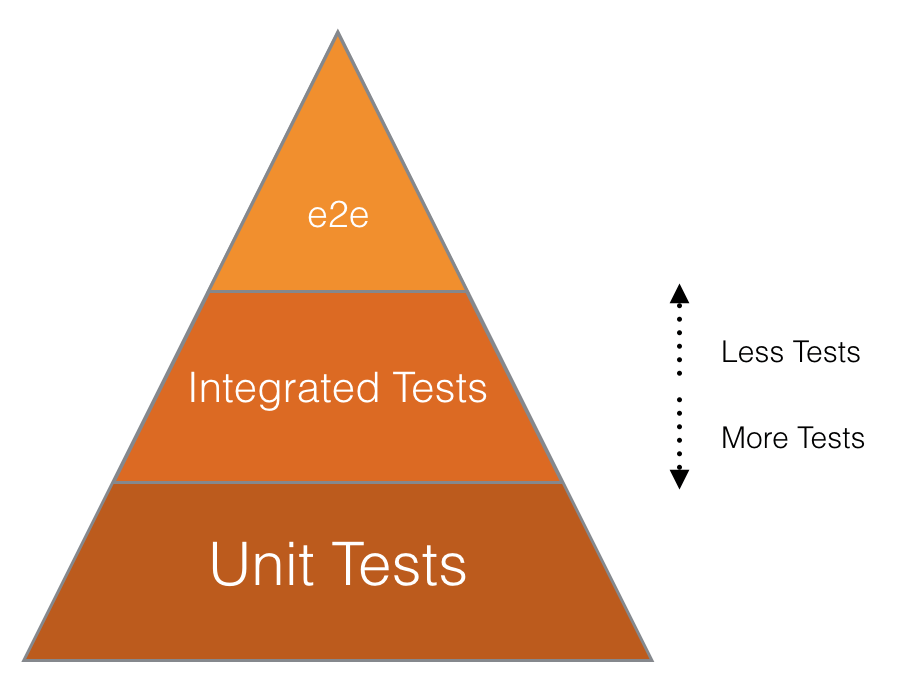
\includegraphics[width=10cm]{images/testing_triangle.png}
    \caption{Piramida testów}
    \label{fig:testing}
\end{figure}

Jak nie trudno było się domyślić znaczną większość testów w kodach programów stanowią testy jednostkowe. Wynika to z dużej popularności metodyki testowania TDD oraz coraz częstszego zauważania przez programistów korzyści wynikających z wykonywania testów. Naturalnym rezultatem chęci zwiększenia procentowego pokrycia kodu testami jest tworzenie większej liczby testów jednostkowych.

Według statystyk opublikowanych przez serwis GitLab\cite{GitLabTesting} testy jednostkowe stanowią na dzień 01.05.2019 71\% wszystkich testów odnalezionych w kodzie. Testy integracyjne oraz White Box pozostają umiarkowanie popularne, natomiast obecność testów Black Box wynosi jedynie 0.17\%.

\begin{center}
\begin{tabular}{ |c|c| } 
 \hline
 Poziom testowania & Ilość testów  \\ 
  \hline
 Testy Black-box (e2e)  & 99 (0.17\%) \\ 
 Testy White-box  & 6440 (10.9\%) \\ 
 Testy integracyjne & 10,577 (17.9\%)  \\ 
 Testy jednostkowe & 41,809 (71\%)  \\ 
 \hline
\end{tabular}
\end{center}

Biorąc pod uwagę, że znaczną większość przeprowadzanych testów stanowią w kodzie testy jednostkowe oraz integracyjne ważne okazują się metody ich automatyzacji. Wykorzystana do tego zostanie praktyka CI - Continuous Integration. 

\subsection{Rola CI w testach}
Zaczynając myślenie o Continuous Integration trzeba najpierw zrozumieć, że nie jest możliwe jednoznaczne zdefiniowanie jak taka ciągła integracja będzie wyglądać w każdym projekcie. Nasze oczekiwania i wymagania od takiej integracji często będą zależne od rodzaju projektu przy którym pracujemy, struktury firmy, wymagań biznesowych od klienta, od faktu czy nasz projekt działa na zasadzie Open Source. Wynika to z faktu, że obecnie ciągła integracja wykorzystywana jest znacznie szerzej niż tylko przeprowadzanie testów w kodzie. 

Ciągła integracja ma pozwolić zespołowi deweloperów na łatwiejsze i bezpieczniejsze tworzenie kodu, podczas którego nie będzie konieczności poświęcania dużej ilości czasu na zarządzanie bazą kodu oraz rozwiązywanie problemów, które wynikają z jednego błędu, a który dotyka dużej części systemu. W praktyce głównym celem do którego dążymy implementując ciągłą integrację jest stworzenie systemu, który po każdym dodaniu kodu do repozytorium będzie uruchamiać wszystkie wyznaczone przez nas testy - zwykle jednostkowe i integracyjne oraz sprawdzi czy dodawany kod spełnia wszystkie narzucone mu wymagania. 

Warto pamiętać, że sam fakt korzystania z systemu zarządzania wersjami, jakim jest git, można potraktować jako ważny element ciągłej integracji. Bez wykorzystania jednego repozytorium kodu dla całego projektu, zarządzanie nim byłoby znacznie bardziej czasochłonne, skomplikowane, a co za tym idzie podatne na powstawanie błędów i różnorakich problemów. Tworzenie projektów przy udziale więcej niż kilku osób mogłoby wymagać więcej czasu na ręczne wysyłanie i łączenie kodu niż samo jego pisanie. 

Jedną z praktyk wykorzystywaną w CI jest częste publikowanie naszych zmian w kodzie do repozytorium. Najczęściej będzie to przynajmniej jeden raz na każdy dzień pracy programisty. Podejście takie sprawia, że łatwiej wykryć jest ewentualne problemy, które mogą pojawić się po naszych zmianach. W przypadku gdy publikowana jest większa ilość kodu, znalezienie przyczyny problemu może byś skomplikowane. Dodatkowo częste publikowanie zmian oznacza, że łatwiej jest połączyć kod pisany w jednym miejscu w pliku przez kilku różnych programistów w procesie "mergowania" zmian. 

Częste publikowanie zmian powoduje też, że kod można łatwiej ze sobą połączyć, w zasadzie jest on zwykle łączony z resztą kodu przez cały swój cykl życia. Aby umożliwić taką sytuację developerzy stają się często pracować tylko na jednej gałęzi deweloperskiej, a gdy nie jest to możliwe wykorzystują gałęzie dedykowane danej funkcjonalności przez jak najkrótszy możliwy czas, aby móc jak najszybciej w jak największym stopniu integrować ich kod z resztą. Dodatkową zaletą szybkiej integracji nowej funkcjonalności jest umożliwienie lepszego i szybszego reagowania na ewentualne zmiany w specyfikacji lub kierunku rozwoju projektu. Stworzona funkcjonalność może być na bieżąco testowana przez osoby odpowiedzialne za tworzenie specyfikacji. W razie zmiany strategii tworzenia projektu będzie można stosunkowo szybko wprowadzić odpowiednie zmiany bez marnowania zbędnie dużej ilości czasu zespołu.

Dużą zaletą wynikającą ze stosowania ciągłej integracji jest znaczne ułatwienie skalowania. Dotyczy to zarówno skalowania projektu jako kod, ale także jako zespół programistyczny. Dobrze przetestowany i przemyślany kod ma szansę być znacznie łatwiej rozbudowywalny od takiego, który nie powstawał w wyniku stosowania dobrych praktyk programistycznych. 

Ułatwienie skalowania zespołu wynika z łatwiejszego wdrażania nowych członków do projektu, dotyczy te szczególnie osób na stanowiskach juniorskich. Kod dodawany przez takie osoby często musiał przechodzić przez recenzję od osoby na stanowisku seniora w celu upewnienia się, że spełnia on oczekiwane standardy. Wykorzystanie Continuous Integration w znacznym stopniu wspomaga taki proces, poprzez wykorzystanie następujących funkcji: 

\begin{itemize}
    \item Automatyczne przeprowadzanie testów 
    
    Jest to podstawowe zadanie praktycznie każdej implementacji Continuous Integration. Zapewnia to możliwość uniknięcia regresji podczas dodawania nowego kodu oraz utrzymywania starego. 
    Platforma na której dokonujemy integracji może zostać skonfigurowana, aby nie pozwolić na dodanie do repozytorium kodu, który nie przejdzie określonych testów. Zwykle będą to wszystkie testy jednostkowe, integracyjne oraz wybrane testy e2e, aktywowane w kodzie przez specjalne flagi, oznaczające elementy projektu, które powinny być poprawnie zaimplementowane. 
    \item Sprawdzanie pokrycia kodu testami
    
    Pokrycie testami ( code coverage ) to bardzo ważna statystyka. Wyraża ona w punktach procentowych jak duża część wyrażeń w naszym projekcie jest testowana. Statystykę tę można wykorzystać, w razie gdyby ktoś próbował dodać do repozytorium nieprzetestowany kod. Oczywiście możliwe jest obejście takiego sprawdzenia poprzez napisanie niepoprawnego testu, który nie wnosi żadnej wartości, jednak w dobrych zespołach programistycznych statystyka jest pomocna jeśli chcemy zachować dobrą jakość pisanego kodu. Istnieją opinie, że pokrycie testami powinno wynosić 100\%, jednak zwykle spotykają się one z opinią, że nie przyniesie to wymiernych rezultatów, ponieważ nawet wtedy w programie mogą znaleźć się błędy logiczne, których nie da się wykryć automatycznymi testami. Zwykle przyjmuje się wartości 80\% - 95\% za odpowiednie przy szacowaniu wymaganego pokrycia kodu. Znalezienie odpowiedniej pracy dla naszego projektu wymaga doświadczenia, znajomości zespołu i zrozumienia wymagań jakie stawia przed nami projekt.
    \item Linting kodu
    
    Lintingiem kodu nazywamy wykorzystanie narzędzie do statycznej analizy kodu. Jego zadaniem w przypadku wykorzystania do ciągłej integracji jest sprawdzanie czy kod, który próbujemy dodać odpowiada standardom wykorzystywanym w projekcie. Może to dotyczyć między innymi tego czy nawiasy otwieramy w nowej linii, konwencji tworzenia nazw zmiennych ( wykorzystanie camelCase, PascalCase, podkreślenia ), definiowania argumentów funkcji w wielu liniach. Z pozoru rola lintingu wydaje się mała, a nawet zbędna, jednakże w dużych projektach, przy których pracuje wiele osób o różnych preferencjach ważne jest tworzenie kodu, który jest jednolity stylistycznie, aby był on spójny i łatwy w czytaniu dla osób, które nie mają z nim dużego doświadczenia.
    \item Integracja z kanałem komunikacji
    
    Wykorzystanie Continuous Integration umożliwia synchronizację naszego repozytorium z wykorzystywanym w projekcie kanałem komunikacyjnym. Obecnie najpopularniejszym wykorzystywanym w profesjonalnych projektach jest Slack, a w projektach tworzonych przez społeczność często także Discord. Integracja taka umożliwia nam otrzymywanie na naszym kanale powiadomień dotyczących repozytorium. Możemy skonfigurować je aby otrzymywać je za każdym razem kiedy nie uda się wykonać testu przy próbie dodania kodu. Możliwe będzie wtedy szybsze naprawienie problemu, jeśli powiadomienie otrzymają odpowiednie osoby i będą mogły szybciej zareagować. Powiadomienia możemy wysyłać też przy poprawnym przejściu testów, co może się przydać jeśli wykonujemy skomplikowane testy, których wykonanie zajmuje więcej czasu. 
\end{itemize}

\begin{figure}[htbp]
    \centering
    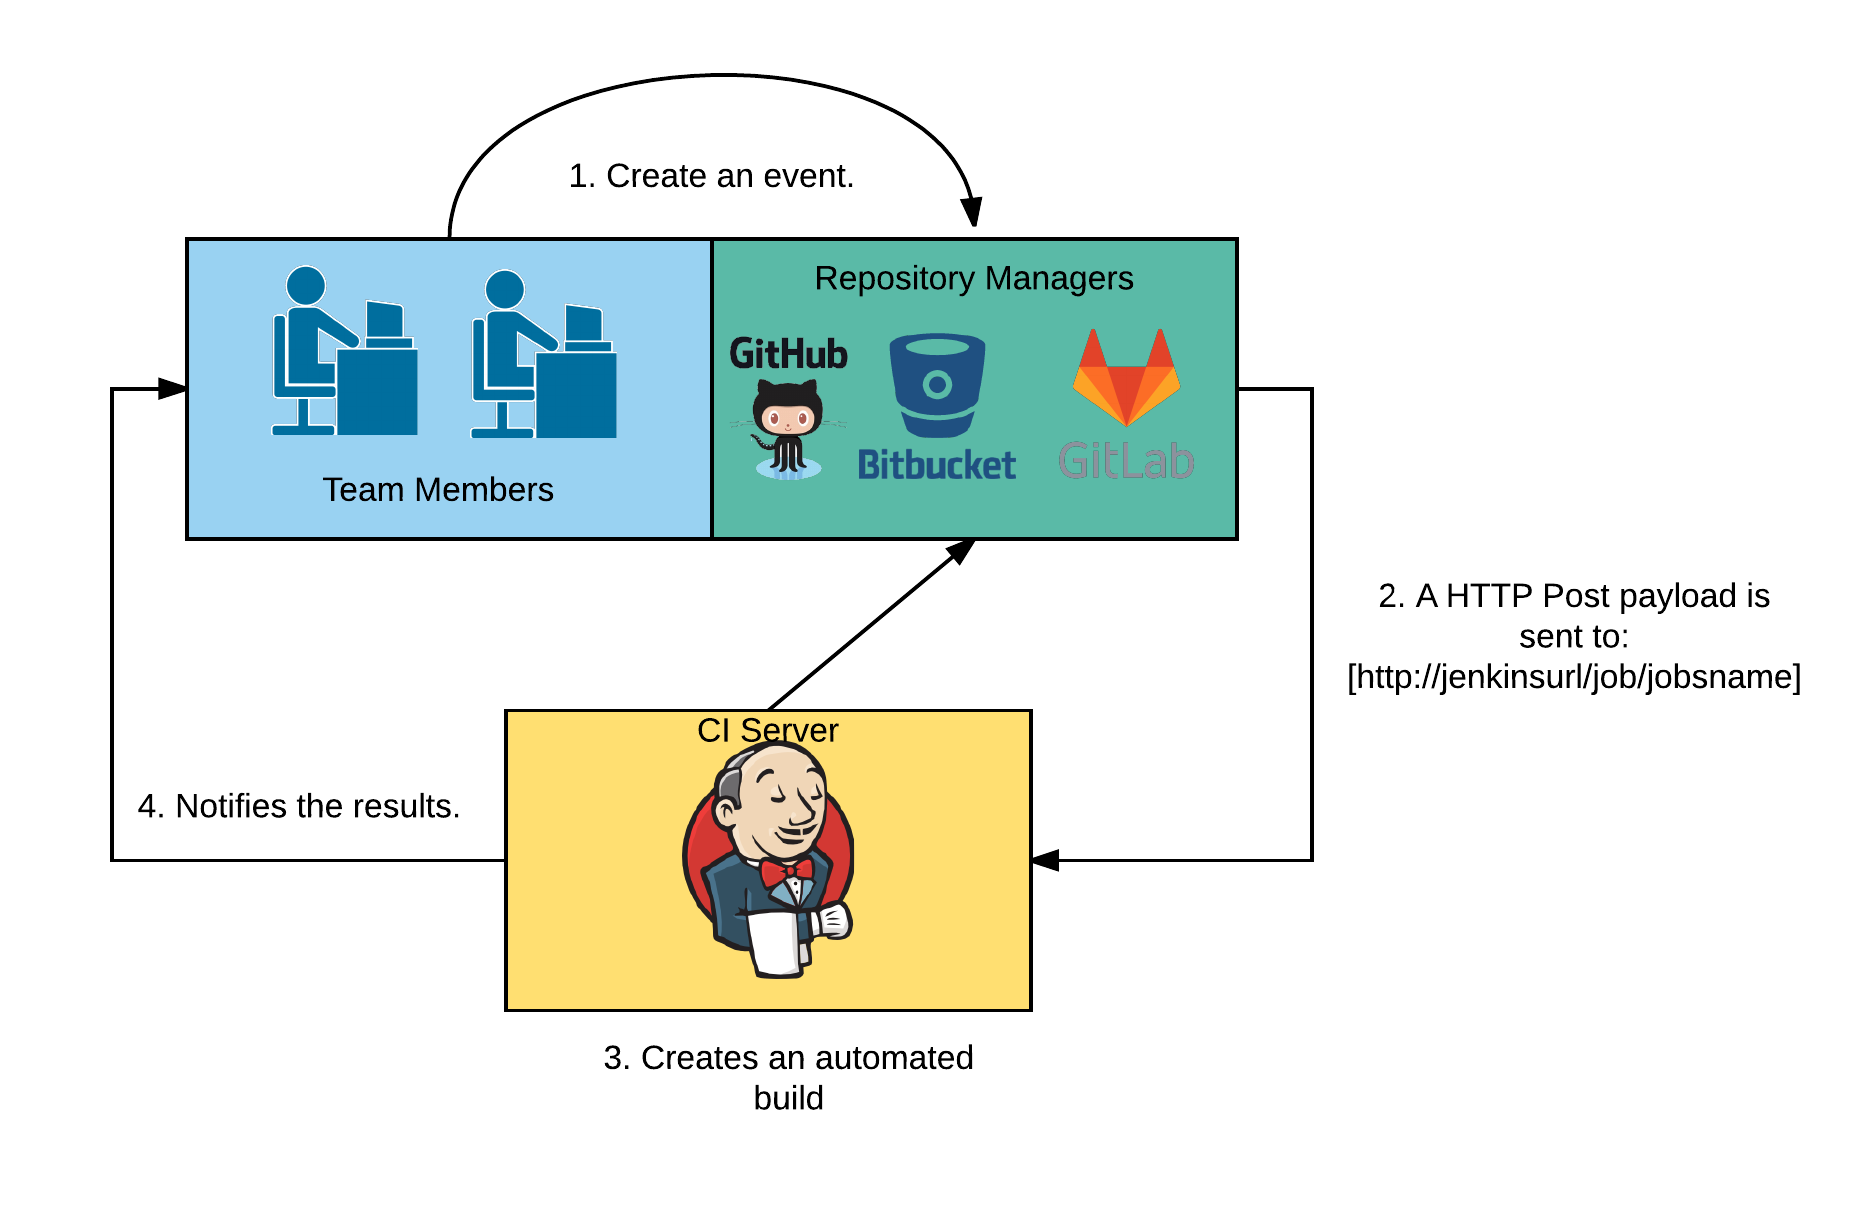
\includegraphics[width=13cm]{images/ci_flow.png}
    \caption{Schemat działania CI, źródło: medium.com/@automationdiscovery}
    \label{fig:ciflow}
\end{figure}

\subsubsection{Wykrywanie błędów bezpieczeństwa}
Dużą korzyścią wynikającą z ciągłej integracji jest możliwość otrzymywania powiadomień dotyczących problemów z bezpieczeństwem w naszym projekcie. Mogą one dotyczyć zarówno błędów wykrytych w wykorzystywanych bibliotekach zewnętrznych jak i przykładowo prywatnych kluczy API, których nie powinniśmy udostępniać publicznie w repozytorium. 

W przypadku wykorzystania platformy GitHub jako repozytorium otrzymujemy alerty o błędach bezpieczeństwa w bibliotekach bez konieczności jakiejkolwiek konfiguracji. 

\begin{figure}[htbp]
    \centering
    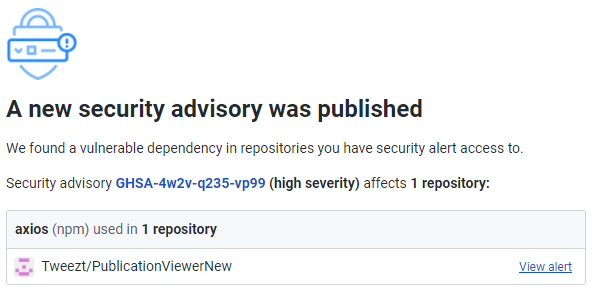
\includegraphics[width=10cm]{images/GitHubAlert.png}
    \caption{Powiadomienie bezpieczeństwa z serwisu GitHub, źródło: własne}
    \label{fig:githubalert}
\end{figure}

Dostępne są także alternatywne serwisy monitorujące repozytoria. Wykorzystanie ich może być konieczne w przypadku projektów komercyjnych, których repozytoria nie są publicznie dostępne. Jednym z popularniejszych jest GitGuardian, który umożliwi nam indywidualne dostosowanie go do potrzeb naszego projektu. 

\begin{figure}[htbp]
    \centering
    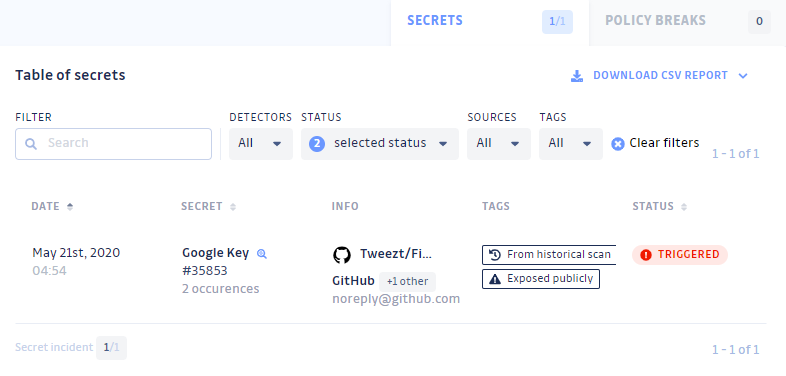
\includegraphics[width=13cm]{images/GitGuardian.png}
    \caption{Powiadomienie bezpieczeństwa z serwisu GitGuardian, źródło: własne}
    \label{fig:gitguardian}
\end{figure}

\subsection{Przykład CI w GitHub Actions}
W celu przetestowania działania różnych funkcjonalności CI do testowania kodu wykorzystamy język python, platformę GitHub oraz oferowaną przez nią usługę GitHub Actions, której działanie zostało już opisane we wcześniejszych częściach pracy.

Nasz projekt spełniać ma następujące założenia: 
\begin{itemize}
    \item Automatycznie wykonywane są wszystkie testy. Do napisania ich wykorzystany zostanie framework pytest. Innym popularnym wyborem dla języka python jest framework unittest. Wybór padł na ten pierwszy ponieważ proste testy można w nim napisać w nieco łatwiejszy sposób, przeszukuje on automatycznie całą bazę kodu w poszukiwaniu testów i umożliwia szybkie uruchomienie ich jedną komendą. Ponadto większość testów pisanych dla unittest zadziała prawidłowo w pytest.
    \item Automatycznie wykonywane jest sprawdzenie pokrycia testami naszego kodu. Wykorzystana zostanie do tego platforma Codecov, która została wybrana z uwagi na łatwą możliwość połączenia z GitHub Actions
    \item Projekt zintegrowany jest z kanałem Slack, na który wysyłane są powiadomienia o działaniach w repozytorium. Slack został wybrany z uwagi na możliwość łatwej integracji z GitHub Actions oraz swoją popularność przy wykorzystaniu w projektach informatycznych. 
\end{itemize}

Pierwszym krokiem było stworzenie repozytorium z kodem i przygotowanymi dla niego testami. 

\begin{figure}[htbp]
    \centering
    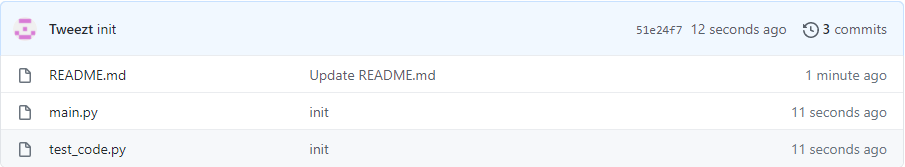
\includegraphics[width=13cm]{images/testingCI1.png}
    \caption{Stworzone repozytorium z przykładowym kodem, źródło: własne}
    \label{fig:ci1}
\end{figure}

\subsubsection{Automatyczne przeprowadzanie testów}
W celu automatycznego wykonywania testów po każdym dodaniu kodu do repozytorium konieczne jest stworzenie tak zwanego workflow. Szczegółowy opis tego zagadnienia został przedstawiony w rozdziale 4.2. 

\begin{lstlisting}[caption={plik main.yaml zawierający workflow automatycznie przeprowadzający testy}]
name: CI
on:
  push:
    branches: [ main ]
  pull_request:
    branches: [ main ]

jobs:
  runtests:
    runs-on: ubuntu-latest

    steps:
      - uses: actions/checkout@v2

      - name: Setup Python
        uses: actions/setup-python@v2.2.1
        with: 
          python-version: 3.8 

      - name: Run tests
        run: |
          pip install pytest
          pytest
\end{lstlisting}

Wykorzystany został w nim system operacyjny Ubuntu w najnowszej wersji oraz język python w wersji 3.8, ponieważ na takiej wersji były przeprowadzane testy lokalne. Samo wykonanie testów odbywa się w dwóch ostatnich liniach. Najpierw instalowana jest biblioteka pytest, a następnie jednym poleceniem uruchamiane są wszystkie zaimplementowane w kodzie testy. 

\begin{figure}[htbp]
    \centering
    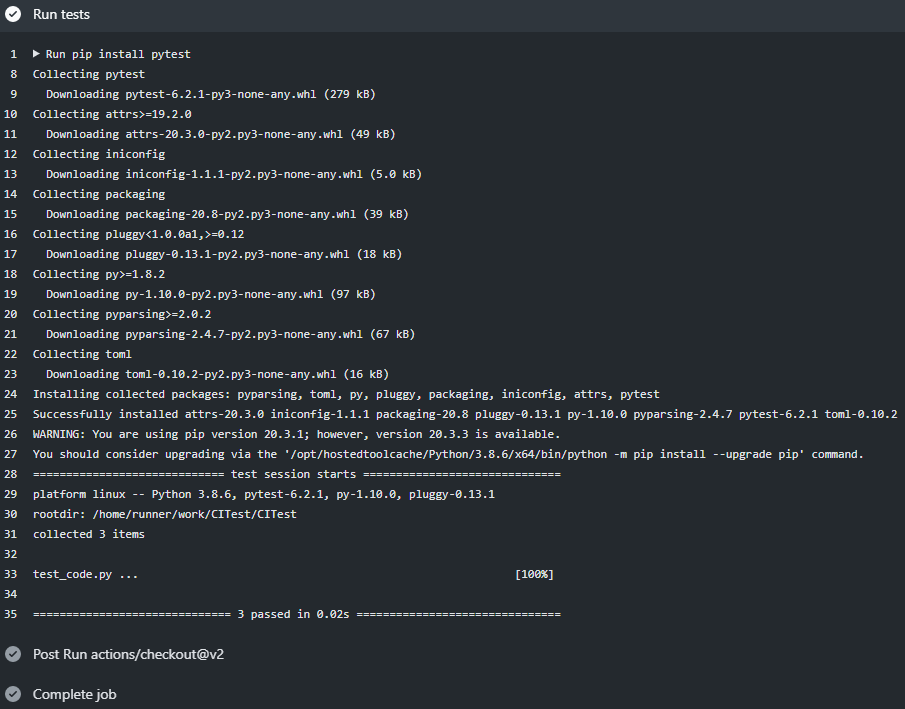
\includegraphics[width=11cm]{images/testingCI3.png}
    \caption{Wynik uruchomionej akcji z testami, źródło: własne}
    \label{fig:ci3}
\end{figure}

Po przejściu do zakładki Actions, można zobaczyć, że testy wykonane zostały poprawnie. 
Po celowym sprawieniu, że test jednostkowy nie powodzi się i opublikowaniu zmian w repozytorium można zobaczyć że jesteśmy o tym informowani w zakładce Actions oraz nad listą plików w repozytorium. 

\begin{figure}[htbp]
    \centering
    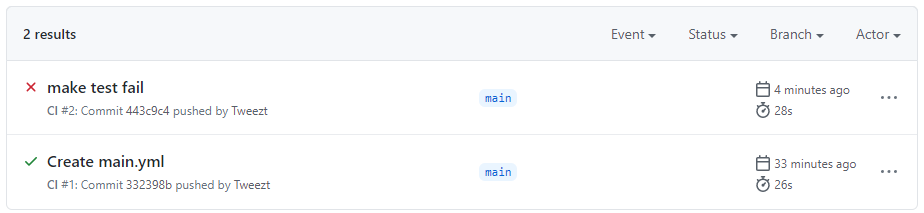
\includegraphics[width=11cm]{images/testingCI4.png}
    \caption{Negatywny wynik testu w zakładce Actions, źródło: własne}
    \label{fig:ci4}
\end{figure}

\begin{figure}[htbp]
    \centering
    
\includegraphics[width=7cm]{images/testingCI5.png}
    \caption{Negatywny wynik testu nad listą plików, źródło: własne}
    \label{fig:ci5}
\end{figure}

\subsubsection{Integracja z serwisem Codecov}
Pierwszym krokiem do przeprowadzenia integracji z serwisem Codecov było zalogowanie się tam przy pomocy konta GitHub, na którym znajduje się repozytorium z projektem. Po udanym zalogowaniu konieczne było pobranie klucza CODECOV\_TOKEN, który należy umieścić w odpowiednim miejscu w ustawieniach repozytorium. Kolejnym krokiem było utworzenie kolejnego pliku .yaml odpowiedzialnego za uruchamianie nowego workflow. 

\begin{lstlisting}[caption={plik coverage.yaml zawierający workflow automatycznie sprawdzający pokrycie testami}]
name: coverage testing
on:
  push:
    branches: [ main ]
    
jobs:
  runtests:
    runs-on: ubuntu-latest
    steps:
      - uses: actions/checkout@v2

      - name: Setup Python
        uses: actions/setup-python@v2.2.1
        with: 
          python-version: 3.8 
      - name: Generate coverage report
        run: |
          pip install pytest
          pip install pytest-cov
          coverage run test_code.py
          coverage report
          coverage xml
      - name: Upload  to Codecov
        uses: codecov/codecov-action@v1
        with:
          token: ${{ secrets.CODECOV_TOKEN }}
          file: ./coverage.xml
          flags: unittests
\end{lstlisting}

Wykorzystywana jest tutaj akcja codecov-action, która pozwala nam w łatwy sposób automatycznie wysłać nasz raport do serwisu. Po prawidłowym wykonaniu wszystkich operacji możemy zobaczyć nasze pokrycie testami w serwisie Codecov.io. 

\begin{figure}[htbp]
    \centering
    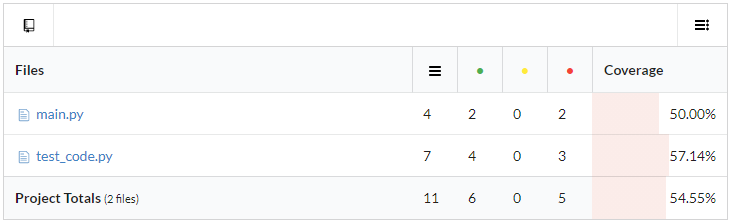
\includegraphics[width=12cm]{images/testingCI6.png}
    \caption{Raport pokrycia kodu testami, źródło: własne}
    \label{fig:ci6}
\end{figure}

\subsubsection{Integracja z kanałem Slack}
Integrację z kanałem Slack można przeprowadzić w sposób analogiczny do integracji z serwisem Codecov, pomocne są tutaj Akcje dostarczone przez te serwisy, które powodują, że konieczna konfiguracja sprowadza się do podania odpowiednich kluczy dostępu. Z tego powodu wykorzystamy odmienne podejście, aby sprawdzić jak można dokonać takiej integracji od strony Slacka. 

Pierwszym krokiem było dodanie aplikacji GitHub do naszego kanału Slack. Można ją znaleźć w galerii aplikacji, dostępnej pod adresem \url{citestingworkspace.slack.com/apps}. Po poprawnym uwierzytelnieniu konta należy wybrać, do których kanałów chcemy dać aplikacji dostęp. 

\begin{figure}[htbp]
    \centering
    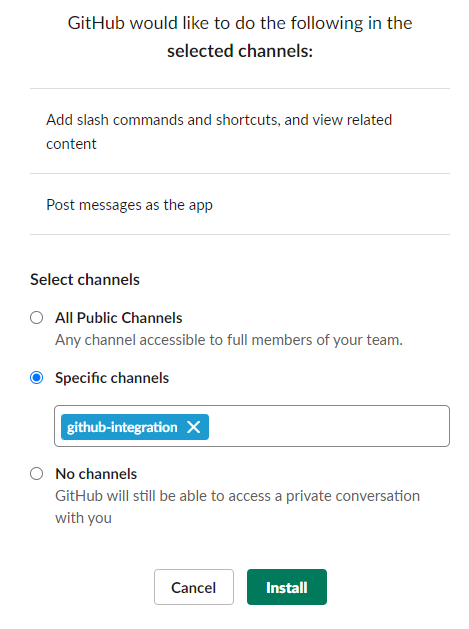
\includegraphics[width=5cm]{images/testingCI7.png}
    \caption{Nadanie aplikacji GitHub uprawnień do korzystania z kanałów, źródło: własne}
    \label{fig:ci7}
\end{figure}
Ostatnim krokiem jak wskazanie aplikacji, z którym repozytorium w serwisie GitHub chcemy ją zintegrować. Odbywa się to poprzez polecenie 
\begin{lstlisting}[caption={Polecenie pozwalające połączyć aplikację GitHub z repozytorium}]
/github subscribe owner/repository
\end{lstlisting}

gdzie owner to nazwa konta, a repository to nazwa naszego repozytorium. 

Po wykonaniu wszystkich kroków i udostępnieniu nowej zmiany w repozytorium możemy zobaczyć powiadomienie wysłane nam przez nowo zainstalowaną aplikację. 

\begin{figure}[htbp]
    \centering
    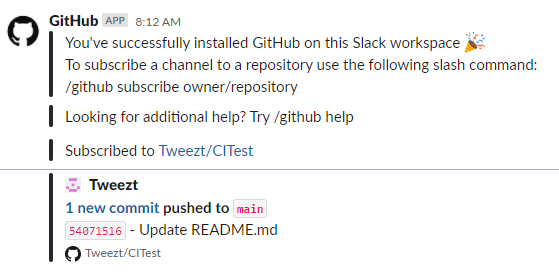
\includegraphics[width=12cm]{images/testingCI9.png}
    \caption{Powiadomienie o nowych zmianach w kodzie w repozytorium, źródło: własne}
    \label{fig:ci9}
\end{figure}

Po wykonaniu wszystkich tych czynności udało nam się stworzyć repozytorium, które dzięki wykorzystaniu ciągłej integracji pozwala na sprawne przeprowadzanie testów, analizę pokrycia nimi kodu oraz umożliwia automatyczne informowanie członków zespołu o zmianach w kodzie. 

